\documentclass[12pt,a4paper]{article}
\usepackage[width=.75\textwidth]{caption}
\usepackage{graphicx}
\usepackage{authblk}
\usepackage{amsmath}
\usepackage{amsfonts}
\usepackage{braket}
\usepackage{epigraph}
\usepackage{amssymb}
\usepackage{amsthm}
\usepackage{bbm}
%\usepackage{mathrsfs}
\usepackage[mathscr]{euscript}
\usepackage[top=2cm, bottom=2cm, left=2cm, right=2cm]{geometry}
\usepackage{fancyhdr}

\theoremstyle{myrule}
\newtheorem{myrule}{Rule}[section]

\theoremstyle{postulate}
\newtheorem{postulate}{Postulate}[section]

\theoremstyle{definition}
\newtheorem{definition}{Definition}[section]


\newtheorem{theorem}{Theorem}[section]
\newtheorem{corollary}{Corollary}[theorem]
\newtheorem{lemma}[theorem]{Lemma}

\setlength{\epigraphwidth}{0.8\textwidth}

\pagestyle{fancy}
\begin{document}

%title and author details
\title{Multi-Observer Quantum Mechanics from Classical Bayesian Inference}
\author[1]{Kevin Player\footnote{kjplaye@gmail.com}}

\maketitle


\epigraph{Solipsism may be logically consistent with present Quantum Mechanics, Monism in the sense of Materialism is not.}{Eugene Wigner}

\abstract{We present several quintessential quantum ideas and shed them in a classical light.  We argue how quantum information theory can be understood as a generalization of classical information theory in a nonstandard way (without density matrices).  In fact, we show how classical information theory can be embedded in quantum information theory using zero phase wavefunctions.  We employ this embedding to motivate a new multi-observer extension of quantum mechanics. Finally, we outline an experiment to test the existence of our multi-observer theory.}

\section{Mathematical Framework}
This section lays out a mathematical foundation for talking about information. The arguments are rather technical and are not required for an appreciation of the main results.  The reader is invited to skip ahead to Section \ref{physicsstart} in a first read through.

Lets start with a 3-bit example, where each bit is realized by coins which are either heads (H) or tails (T).  With these 3 coins in hand, we conduct some thought experiments.  During this section we outline an epistemic treatment of classical information where we represent our classical knowledge of the 3 coin ensemble. The ideas that we encounter all extend without loss of generality to $n$-bits or any finite set.

\subsection{Tribits and Notation}
Let us describe the situation once we throw the 3 coins.  We move freely between binary bits ($0$ and $1$) and coin states ($H$ and $T$) mapping between them $H \leftrightarrow 0$ and $T \leftrightarrow 1$. Let
\[
x_i \in \{H,T\}
\]
be the outcome for the throws $i$ = $1,2,3$ and let $x = (x_1, x_2, x_3)$ denote the resulting sequence or tribit.  There are 8 tribits and we will refer to them with the italic integers $\mathit{0}$ through $\mathit{7}$ in binary order.  Let $C$ be the set of 8 possible tribits
\[
 C = \{HHH,HHT,\cdots,TTH, TTT\} = \{\mathit{0},\cdots,\mathit{7}\}
\]
  
\subsection{Postulates for Constructing Knowledge Statements}
For any set $A$, let $\mathcal{K}(A)$ be the set of knowledge statements about $A$.  Motivating by example, we construct and present knowledge statements $\mathcal{K}(C)$ for $C$.  We do this by repeatedly applying the following simple postulates.
\begin{postulate}
\label{rule1}
For any tribit $x \in C$ we have the knowledge statement $b_x \in \mathcal{K}(C)$, that says we know $x$ with certainty or probability 1.  We call this a basic statement.
\end{postulate}
There are 8 tribits, so there are 8 basic statements, $b_\mathit{0},\cdots,b_\mathit{7}$.  Each statement is a separate kind of knowledge about the tribit.  A physical constraint is that an observer can only hold one knowledge statement at any given time.  In contrast, a knowledge statement itself may represent more than one possibility simultaneously, as is the case in the next Postulate.
\begin{postulate}
 \label{rule2}
  A formal superposition can be made for any statements $s_1 \in \mathcal{K}(C)$ and $s_2 \in \mathcal{K}(C)$ and $\alpha \in [0,1]$
  \begin{equation}
  \label{super}
  \text{super}_\alpha(s_1,s_2) = \alpha s_1 + (1 -\alpha) s_2.
  \end{equation}
This formal combination means to take statement $s_1$ with probability $\alpha$ and statement $s_2$ with probability $(1-\alpha)$; This is a new statement in $ \mathcal{K}(C)$.
\end{postulate}

\subsection{Distributions on the Ensemble}

For any set $A$ let $\mathcal{P}(A)$ be the set of probability distributions on $A$.  Then $\mathcal{P}(C)$ is the set of probability distributions on tribits. For a fixed $\eta \in \mathcal{P}(C)$ we let $p_i(\eta)$ be the probability of seeing the tribit $i$ under $\eta$.  For an example, consider the tribit $\mathit{6} = TTH$.  $p_\mathit{6}$ is the probability of seeing $\mathit{6}$ under $\eta$.

The eight $p_i$ completely characterize $\eta$ as the vector $(p_\mathit{0}(\eta),\cdots,p_\mathit{7}(\eta)) \in \mathbb{R}^8$.  Call this 8 dimensional ambient space $\mathcal{V}(C)$. In general $\mathcal{V}(A) = \mathbb{R}^A$ for the set $A$.  We identify any $a \in A$ with the basis element $b_a$.  In this way we map $A \hookrightarrow \mathcal{V}(A)$.
\begin{lemma}
\label{prob}
  $\mathcal{K}(C)$ = $\mathcal{P}(C)$
\end{lemma}
\begin{proof}
  Let $\eta \in \mathcal{K}(C)$.  The Postulates \ref{rule1} and \ref{rule2}, that form $\eta$, output probability distributions at every step.  So $\eta \in \mathcal{P}(C)$.
  
  WLOG we can assume that $p_0 \not = 0$.  Let $\eta = (p_i) \in \mathcal{P}(C)$.  We inductively extend the distribution
  \[
  \eta_k = \gamma_k (p_0, \cdots, p_{k-1}, 0, \cdots, 0)
  \]
  to
  \[
  \eta_{k+1} = \gamma_{k+1} (p_0, \cdots, p_{k}, 0, \cdots, 0)
  \]
  using basic $b_k$ and 
  \[
  \eta_{k+1} = super_\alpha(\eta_k,b_k)
  \]
  for appropriate choices $\alpha$ and of normalizations $\gamma_k, \gamma_{k+1}$. So we have applied a sequence of Postulates that form $\eta$ and hence $\eta \in \mathcal{K}(C)$.
\end{proof}

\begin{corollary}
  For any finite set $A$,
  \[
  \mathcal{K}(A) = \left\{ (p_a)_{a \in A} \in \mathbb{R}^{A} \middle | \sum_{a \in A} p_a = 1 \right\}  \subseteq \mathcal{V}(A)
  \]
where $\mathcal{K}(A)$ is affine codimension 1 in $\mathcal{V}(A)$ and $\mathcal{V}(A)$ is the vectorspace $\mathbb{R}^A$.
\end{corollary}
\begin{proof}
  The right hand side is the definition of $\mathcal{P}(A)$ and the claim follows using a generalization of the proof of Lemma \ref{prob}.
\end{proof}

A general knowledge statement $\eta \in \mathcal{K}(C)$ combines the basic statements $b_\mathit{0}, \cdots, b_\mathit{7}$ using coefficients $p_\mathit{0}, \cdots, p_\mathit{7}$,
\[
  p_\mathit{0},\cdots,p_{\mathit{7}} \in \mathbb{R}^+,
\]so that $\eta = \sum p_i b_i$.  To be a statistical distribution we also need it to be normalized with $\sum p_i = 1$.  Note that now (\ref{super}) is more than just a formal relation since it actually holds linearly inside of $\mathcal{V}(C)$.


Let $\mathcal{S}$ be the category of sets.  Let $\mathcal{W}$ be the category of real vectorspaces.  Then
\begin{lemma}
$\mathcal{V}$ is a contravariant functor from $\mathcal{S}$ to $\mathcal{W}$ that takes injections and surjections to surjections and injections respectively.
\end{lemma}
\begin{proof}
  Let $f:A \hookrightarrow B$ be an injection. Consider the map for $b \in B$ to $\mathcal{V}(A)$ to be as follows
  \[
     b \mapsto \left\{ \begin{array}{cc} b & \text{ if } b \in A \\ 0 & \text{ if } b \not \in A  \end{array} \right.
\]
We extend this map linearly to form the orthogonal projection $\mathcal{V}(f):\mathcal{V}(B) \twoheadrightarrow \mathcal{V}(A)$.

Now let $g:A \twoheadrightarrow B$ be a surjection.  Consider the map for each $b \in B$ to the sum over the fiber of $b$
  \[
  b \mapsto \sum_{a \in g^{-1}(b)} a.
  \]
We linearly extend this to the map $\mathcal{V}(g):\mathcal{V}(B) \hookrightarrow  \mathcal{V}(A)$.  Each of these fibers is disjoint so the map is injective.

  Consider a general map $h:A \rightarrow B$.  We write this map as a surjection onto the image followed by an injection  $A \twoheadrightarrow Im(h) \hookrightarrow B$.  We then send $h$ to
 \[
 \mathcal{V}(A) \hookleftarrow \mathcal{V}(Im(h)) \twoheadleftarrow \mathcal{V}(B).
 \]
  Finally, we examine the composition of $r:A \rightarrow B$ and $s:B\rightarrow D$.  For any $d \in D$ we have three possibilities
  \begin{enumerate}
  \item $d \not \in Im(s)$
  \item $d \in Im(s)$, but $s^{-1}(d) \cap Im(r) = \emptyset$
  \item $d \in Im(s \circ r)$
  \end{enumerate}

\begin{figure}[h]
\centering
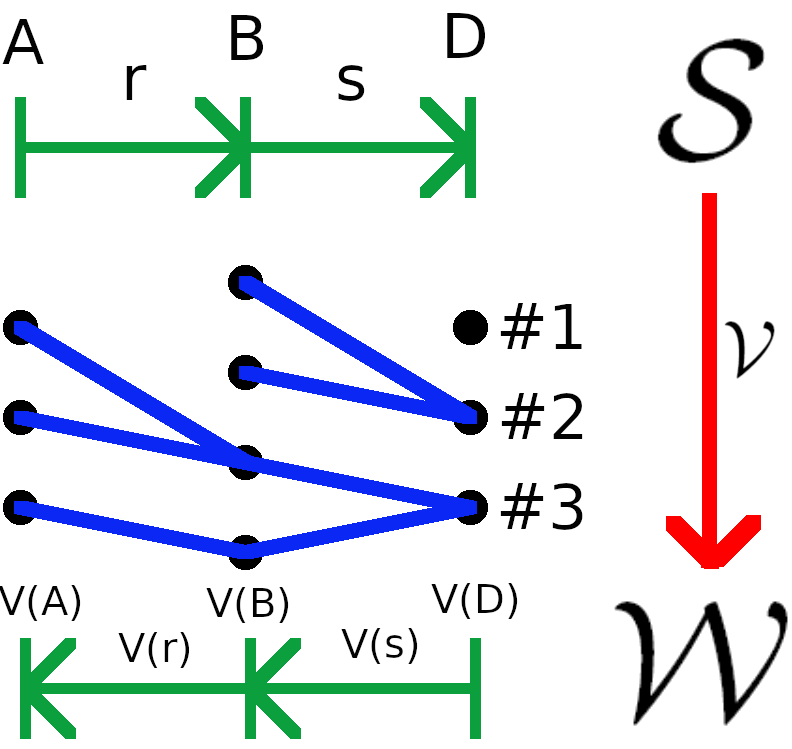
\includegraphics[scale=1.0]{functor.png}
%\caption{Three cases for $s \circ r$}
\end{figure}
  
  We wish to show the composition property of the functor, $\mathcal{V}(s \circ r) = \mathcal{V}(r) \circ \mathcal{V}(s)$, by conidering the three above possibilites on a case by case basis.  Consider possibility \#1.  In this case we have $\mathcal{V}(s)$ sending $d$ to zero.  For possibility \#2, $\mathcal{V}(s)$ sends $d$ to a sum over the fiber of $d$ under $s$, but then all of $s^{-1}(d)$ gets sent to zero by $\mathcal{V}(r)$.  For possibility \#3, $\mathcal{V}(s)$ sends $d$ to the sum over $s^{-1}(d)$ and then that gets sent by $\mathcal{V}(r)$ to the sum over the nonempty $r^{-1}(s^{-1}(d))$.  These cases and behaviors are the same as directly considering $\mathcal{V}(s \circ r)$ where the cases \#1 and \#2 have $d$ getting sent to zero and case \#3 defines the same map as the composition since the fibers under $r$ of the fibers under $s$ are just the fibers under $s \circ r$.

  This demonstrates the composition property of the functor, $\mathcal{V}(s \circ r) = \mathcal{V}(r) \circ \mathcal{V}(s)$.
\end{proof}

Each coin corresponds to a 2 dimensional space $\mathcal{V}(\{H,T\})$ which we will call $V_2$.  The 8 dimensional space $V_2 ^ {\otimes 3}$ has a basis with vectors like $T \otimes H \otimes T$.  Then $\mathcal{V}(C)$, is identified with the tensor power $V_2^{\otimes 3}$ by linearly extending
\[
(x_1,x_2,x_3) \mapsto x_1 \otimes x_2 \otimes x_3.
\]

\begin{lemma}
\label{product}
  $\mathcal{V}(A \times B) = \mathcal{V}(A) \otimes \mathcal{V}(B)$ and the $n$-bit knowledge space $\mathcal{V}(\mathbb{Z}_2^n)$ is $V_2 ^ {\otimes n} \cong \mathbb{R}^{2^n}$.  $\mathcal{V}(A \times B \twoheadrightarrow A)$ identifies $\mathcal{V}(A)$ with $\mathcal{V}(A) \otimes \mathbbm{1}_B$.  The same is true for $B$ and $\mathbbm{1}_A$.
\end{lemma}
\begin{proof}
  We map the $|A|\cdot|B|$ basis elements $(a,b) \mapsto a \otimes b$.  The linear extension of the map is an isomorphism.  For $n$-bits we repeatedly apply the map to get the formula for $\mathcal{V}(\mathbb{Z}_2^n)$.  For the last expression write $\mathbbm{1}_B := \sum_{b \in B} b$ then the sum over the fiber of $a \in A$ is $a \otimes \mathbbm{1}_B$.  The same argument applies when reversing $a$ and $A$ with $b$ and $B$.
\end{proof}

\section{Classical Information Theory}
\label{physicsstart}
We are ready to enter into the physics surrounding knowledge statements.  This means we are going to start talking about measurement and observation.  This is part of our epistemic program.  We will take a Bayesian viewpoint that knowledge is updated by observation.

\subsection{Classical Bayesian Projections}
\label{proj}
Let us go back to our three coin toss example with eight tribits $C$.   We consider knowledge statements about the three coins $\mathcal{K}(C)$ in an eight dimensional ambeient space $\mathcal{V}(C)$ where $C$ is a basis.  We don't always get to measure the exact tribit.  For instance, we might only get to know that the first coin is $T$ and that the 2nd and 3rd coins are the same.  This corresponds to an exemplar subset of $C$, which we will call $S$
\[
\begin{split}
  S &= \{s \in C | x_1 = T, x_2 = x_3 \} \\
    & = \{\mathit{4},\mathit{7}\} \hspace{0.4 in} \text{(THH, TTT)}
\end{split}
\]
We will use $S$ as an example in the remaining text.

\begin{figure}[h]
\centering
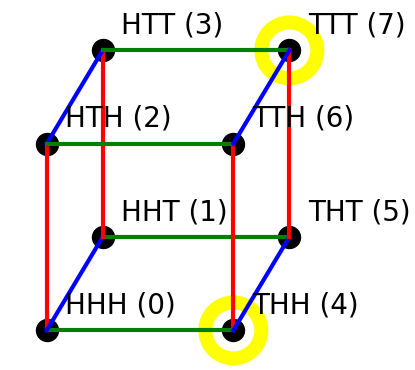
\includegraphics[scale=0.6]{cube.png}
\caption{Coin sequences with $S$ circled in yellow.}
\end{figure}

Someone could make a measurement that tells them that the tribit is in $S$ and nothing else.  This would be a specific case of what we will call a projection measurement, $\rho$, that updates our knowledge to be in $S$.  The statement becomes zero exactly on tribits $i$ where $i \not \in S$ and renormalizes $p_i$ on the remaining $i \in S$.  Specifically we have for the example on $S$, 
\begin{equation}
\label{sdist}
\rho: (p_0,\cdots,p_7) \mapsto \left(0,0,0,0, \frac{p_4}{p_4 + p_7},0,0,\frac{p_7}{p_4 + p_7}\right)
\end{equation}
In more generality we have
\begin{definition}[Bayesian Projection]
\label{projdef}
For any finite set $A$ with $B \subseteq A$ we consider a measurement of $B$.  It takes
\[
p_a \mapsto \left\{ \begin{array}{cc} 0 &\text{ when } a \not \in B \\ \frac{p_a}{\sum_{b \in B} p_b} & \text{ when } a \in B \end{array} \right.
\]
We call this a Bayesian projection since the ambient spaces follow a projection $\mathcal{V}(B \hookrightarrow A)$.
\end{definition}
\subsection{Classical Bayesian Inference}
A more general type of measurement is a probabilistic measurement.  Someone could learn that there is a 95\% chance that the tribit is in $S$.  In full generality we will call such a probabilistic observation $\mathcal{O}$.  We can figure out how to update our knowledge statement from $p_i$, to $\hat{p_i}$, using a relative\footnote{In the ratio, the contribution of $P(\mathcal{O})$ is canceled out and accounted for during normalization.  $P(\mathcal{O})$ only holds significance prior to its observation and it doesn't require consideration during the update process.} version of Bayes's rule
\[
  \frac{\hat{p_i}}{\hat{p_j}} = \underbrace{\frac{P(i | \mathcal{O})}{P(j | \mathcal{O})}}_\text{Posterior}
                              = \underbrace{\frac{P(\mathcal{O} | i)}{P(\mathcal{O}|j)}}_\text{Bayes Factor}  \hspace{0.07 in}  \underbrace{\frac{p_i}{p_j}}_\text{Prior}
\]
Pulling out the Bayes factor we find that we just multiply by the likelihood and re-normalize by $\gamma$
\begin{equation}
\label{inference}
  \hat{p_k} =  \gamma P(\mathcal{O} | k) \hspace{0.07 in} p_k.
\end{equation}
\begin{definition}[Bayesian Inference]
\label{infdef}
  An update of the form (\ref{inference}) is called a Bayesian inference.
\end{definition}
\begin{corollary}
A special case are two-leveled projections $P(\mathcal{O} | k) \in \{0,v\}$, for a fixed value $v$ determined by normalization.  These are the Bayesian projections from Definition \ref{projdef}.
\end{corollary}

\subsection{Classical Correlation}
We consider the uniform distribution on $S$.
\[
\frac{1}{2}(T \otimes H \otimes H) + \frac{1}{2}(T \otimes T \otimes T)
\]
We know the first coin is T, which we give to Eve.  She does nothing with her coin.

We have $HH$ or $TT$ with equal probabilities for the second and third coins.  If we give the second coin to Alice and the third coin to Bob then we have a classical correlation.  If Bob finds that the third coin is $T$ then we know that Alice will also find that the second coin is $T$ (and similarly for $F$).  The reduction is purely epistemic, it is the separate knowledge of Alice and Bob that is changing.

\begin{definition}[Classical Correlation]
\label{corrdef}
In general consider $A \times B$ with surjections $f_A$ and $f_B$ onto $A$ and $B$ respectively.  Consider the set of knowledge statements that factor as coordinate-wise products of $\mathcal{V}(f_A)$ and $\mathcal{V}(f_B)$.  From Lemma \ref{product} we see that such a product must be of the form
\[
(\mathbbm{1}_A \otimes \eta_B) (\eta_A \otimes \mathbbm{1}_B) = \eta_A \otimes \eta_B
\]
where $\eta_A \in \mathcal{K}(A)$ and $\eta_B \in \mathcal{K}(B)$.  We call all other nonfactorable statements ``correlated'' since they do not directly come from knowledge statements of $A$ and $B$ independently.  A simple example uses two bits with the following knowledge statement
\begin{equation}
\label{classiccorr}
  \frac{1}{2} (H \otimes H) + \frac{1}{2} (T \otimes T) 
\end{equation}

\end{definition}

\section{Quantum Information Theory}
\subsection{Classical to Quantum Embedding}
General quantum information\footnote{We are purposely leaving out density matrices and POVMs and just dealing with pure states.} about 3-qubits can be expressed as a wave function.
\[
   q_\mathit{0},\cdots,q_\mathit{7} \in \mathbb{C}
\]
with $\sum |q_i|^2 = 1$.  The Born rule is ostensibly a map $q_i \mapsto |q_i|^2 = p_i$ to classical probability.  In the following subsections we will instrument all of the classical information theoretic constructs from the previous section by restricting the phase\footnote{We consider negative values as 180 degrees out of phase, so zero phase means non-negative real.} of $q_i$ to be zero.  We can map backward $p_i \mapsto \sqrt{p_i} = q_i$; which commutes with the Born rule (subject to normalization):

{
\renewcommand{\arraystretch}{0.1}
\[
\text{(Quantum)} \hspace{0.3 in}
\mathbb{C}^n \begin{array}{c} \twoheadrightarrow \\ \hookleftarrow \end{array}
(\mathbb{R}_{\ge 0})^n
\hspace{0.3 in} \text{(Classical)} 
\]
}

In doing so, we will see that quantum information theory needs to generalize the classical.  In particular we will see that quantum measurement and entanglement restrict to classical measurement and classical correlation for zero phase.

\subsection{Quantum Bayesian Projection}
We illustrate zero phase Bayesian projection with an example.  For the example we define a projection operator $\pi$ which projects onto the space generated by the subset $S$, from the previous subsection
\[
\pi = \sum_{i \in S} \ket{i} \bra{i}.
\]
Then let $A$ be any operator with an eigenspace, with eigenvalue $\lambda$, equal to the image of $\pi$.  An observation of $\lambda$ would correspond to an application of $\pi$, which is a Bayesian projection as in Definition \ref{projdef}.
\begin{theorem}
  The set inclusion $B \subseteq A$ yields a Bayesian Projection as in Definition \ref{projdef}.  Then a zero phase wavefunction instruments the classical measurement.
\end{theorem}
\begin{proof}
Let $q_i = \sqrt{p_i}$ be a zero phase wavefunction corresponding to $(p_i) \in \mathcal{K}$.  Let
  \[
  \lambda_i = \left\{ \begin{array}{ll} 1 \text{ if } i \in B \\ 2 \text{ if } i \not \in B \end{array} \right.
  \]
and define an operator
\[
  D = \sum_{i \in A} \lambda_i \ket{i} \bra{i}
\]
If we make a measurement of $1$, in $D$, then the wave function collapses by projecting onto the eigenspace of $1$. The wave function is then renormalized.  This projection on the $B$-space and normalization of $q_i$ exactly matches the classical Bayesian projection and normalization of $p_i$.
\end{proof}
\subsection{Quantum Bayesian Inference}
\begin{theorem}
  Let $P(\mathcal{O} | i)$ define a Bayesian inference as in Definition \ref{infdef}.  Then a zero phase wavefunction instruments the classical measurement.
\end{theorem}
\begin{proof}
Consider, in the fashion of \cite{nielsenchuang}, a more general measurement with matrix $M_\mathcal{O}$ which is diagonal with entries
\[
   M_\mathcal{O}(i,i) = \sqrt{P(\mathcal{O} | i)}
\]
This measurement is identical to the classical Bayesian inference for zero phase wavefunctions.
\end{proof}

\subsection{Quantum Entanglement}
\begin{theorem}
  Classical correlation knowledge statements become entangled zero phase wavefunction.
\end{theorem}
\begin{proof}
  The example (\ref{classiccorr}) in Definition \ref{corrdef} maps to
  \[
  \frac{1}{\sqrt{2}} (H \otimes H) + \frac{1}{\sqrt{2}} (T \otimes T)
  \]
which is a entangled Bell state.  In general, the correlated knowledge statements are exactly the zero phase entangled states.
\end{proof}
\subsection{Entropy}
Von Neumann entropy is left out of this note since it is not a generalization of classical entropy in the embedding presented here.  This is because the zero phase classical wavefunctions are pure states which all have zero Von Neumann entropy, but the classical entropy is nonzero for all non-basic statements.

\section{Overview of the Generalization}

The quantum mechanical concepts wave function collapse, entanglements and ensembles are generalizations of the classical information theoretic concepts of Bayesian inference, correlation and statistical ensembles respectively.  This is not to say that they are not strange, but to say that they need to be generalizations of the classical concepts.  Wave function collapsing should generalize Bayesian inference and classical measurement.  Entanglement should be a generalization of classical correlation.  This is enough to motivate new ways of doing quantum mechanics, which we will encounter in the next sections.

\subsection{Multi-Observer Quantum Mechanics}
We focus on quantum wave function collapse as a generalization of classical Bayesian inference.  We can implement the classical Bayesian inference within zero phase quantum mechanics as outlined above.  So the classical Bayesian theory has a direct tie in; that observation and measurement occur in tandem with a change in knowledge\footnote{This change in knowledge is tangible, it always occurs as a transfer of matter/energy from the environment to the observer \cite{thrust}.}.  

In the classical theory, knowledge is local to the observer\footnote{Note that current quantum theory is a theory of one observer, usually the experimenter in a lab.  An immediate subject is quantum key distribution(QKD), which requires at least three observers, Alice, Bob, and Eve; the security of QKD depends on multi-observer quantum ontology.}, multiple observers each have their own knowledge.  For instance, Wigner's friend and Wigner each have their own classical knowledge.  It would seem then that Wigner's friend and Wigner must have different zero phase wavefunctions as well, if they are to be generalizing classical knowledge.  This is our prediction for multi-observer quantum physics, that every observer has a local wavefunction. 

\subsection{Prediction and Experiment}

We predict that multi-observer quantum mechanics will be required for a proper generalization of classical knowledge.  We propose an experiment where we inject an ``observer'' into a quantum eraser\footnote{Here we probe the boundaries of what constitutes an observer and a measurement.  We claim that all versions of observer and measurement will be detectable in this experiment whenever it can be done.}.  The injected observer will have to be a small apparatus that is
\begin{itemize}
   \item able to record a measurement $\psi$ of the eraser particle path.
   \item able to forget the measurement $\psi$.
   \item able to demonstrate that a measurement was made with a record $\rho$.
\end{itemize}
Let $\phi$ be the lab technician's wavefunction.  In $\phi$ the apparatus is entangled with the subject particles in the eraser experiment.  We need to find out if there is another wavefunction in play that is not just part of $\phi$.  The key here is that the apparatus is able to demonstrate that it ``knew'' something, or in other words that another wavefunction $\psi$ existed, using $\rho$.

The apparatus can not keep $\psi$ for proper erasure, but must ``forget'' it.  Observed erasure, via an interference pattern, proves that $\psi$ is not a part of $\phi$.  Finally, there should be a record $\rho$ in the apparatus that it did at one point in time record a measurement $\psi$.  Receipt of the report $\rho$ and eraser interference pattern together show that $\psi$ and $\phi$ were necessarily part of a two-observer system.

\section{Acknowledgments}
Thanks to Erik Ferragut and Dan Justice for useful discussions.

\bibliographystyle{ieeetr}
\bibliography{bibliography}

\end{document}
